\documentclass[12pt]{report}
%% Language and font encodings
\usepackage[francais]{babel}
\usepackage[utf8]{inputenc}
\usepackage[T1]{fontenc}
\usepackage{lmodern}
\usepackage[official]{eurosym}

%% Sets page size and margins
\usepackage[a4paper,top=3cm,bottom=2cm,left=3cm,right=3cm,marginparwidth=1.75cm]{geometry}

%% Useful packages
\usepackage{amsmath}
\usepackage{graphicx}
\usepackage[colorinlistoftodos]{todonotes}
\usepackage[colorlinks=true, allcolors=blue]{hyperref}

\title{Projet Licence ADSILLH 2017/2018\\Rapport}
\author{Pierre Antoine Rouby - Lunix}

\date{Année 2017/2018}

\begin{document}
\maketitle

\begin{abstract}
Ce document présente notre projet bigdata.
\end{abstract}

\tableofcontents

\chapter{Le Projet}
\section{Les besoins}
Aujourd'hui pour acheter un bien immobilier il y a deux solutions principal:
\begin{itemize}
\item Passer par du particulier à particulier (leboncoin),
\item Passer par une agence immobilière.
\end{itemize}
La première solution permet d'éviter les frais d'agence, mais il faut avoir
confiance en la personne qui vend le bien.
En effet le cadre juridique et moins plus permissif dans le cas ou il n'y à pas
d'agence.
Il faut donc faire 2 fois plus attention au arnaque et vise cacher.

\section{Solution}
Nous avons donc réfléchie à une solution pour réduire les coups d'agence avec
de la dématérialisation des visites et de l'automatisation de l'estimation des
biens.

Il serrai en effet possible de déterminé automatiquement la valeur d'un bien
en fonction de sa géolocalisation, de ses plans et de plusieurs autre facteur.

La géolocalisation permettrai de connaître les commerces, les transports en commun
et tous autre services à proximité, mais aussi via le registre de cadastre
\footnote{Registre des cadastre français : \url{https://cadastre.gouv.fr/scpc/accueil.do}}
de connaître la valeur des biens vendu résament dans les allant tours.

Les plans quand à eux serve à connaître la surface du bien, mais pour un véritable
estimation il faut aussi prendre en compte l'état actuelle des mures, sols,
plafond, port, etc. Pour cela nous pouvons imaginé utilisé une caméra à 360 à
fin de modélisé l'appartement en 3D. Ses images pourrons aussi servir a faire des
visites de l'appartement avec un casque VR (Virtual Reality).
%% Add images

On peut imaginé utilisé du ``machine learning'' pour le calcule d'un bien, mais
il est aussi possible de simplement appliquer une formule de calcule prés
déterminer.

\chapter{Architecture Big Data comme solution}
\goodbreak

\section{Infrastructure}
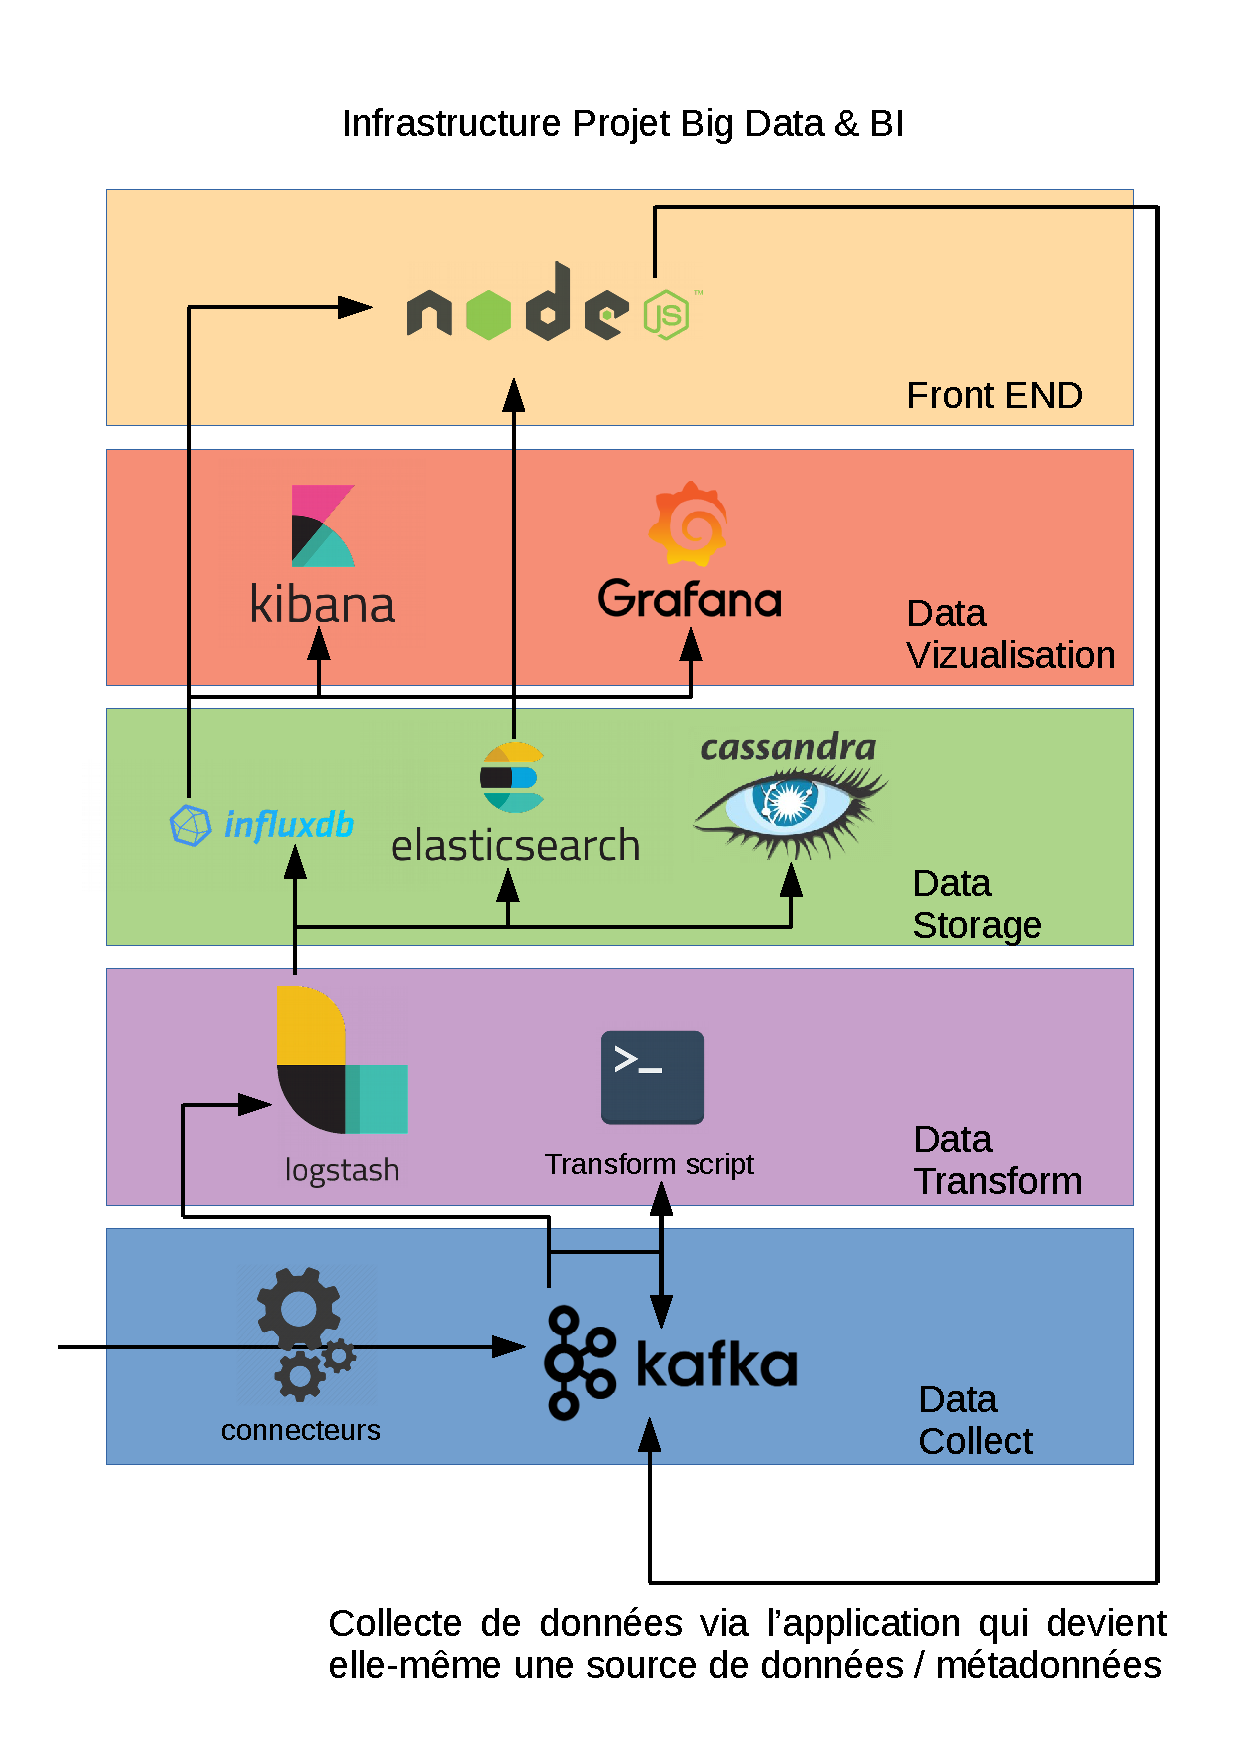
\includegraphics[width=16cm]{pdfinc/SchemaInfra.pdf}

\goodbreak

\section{Présentation des outils}
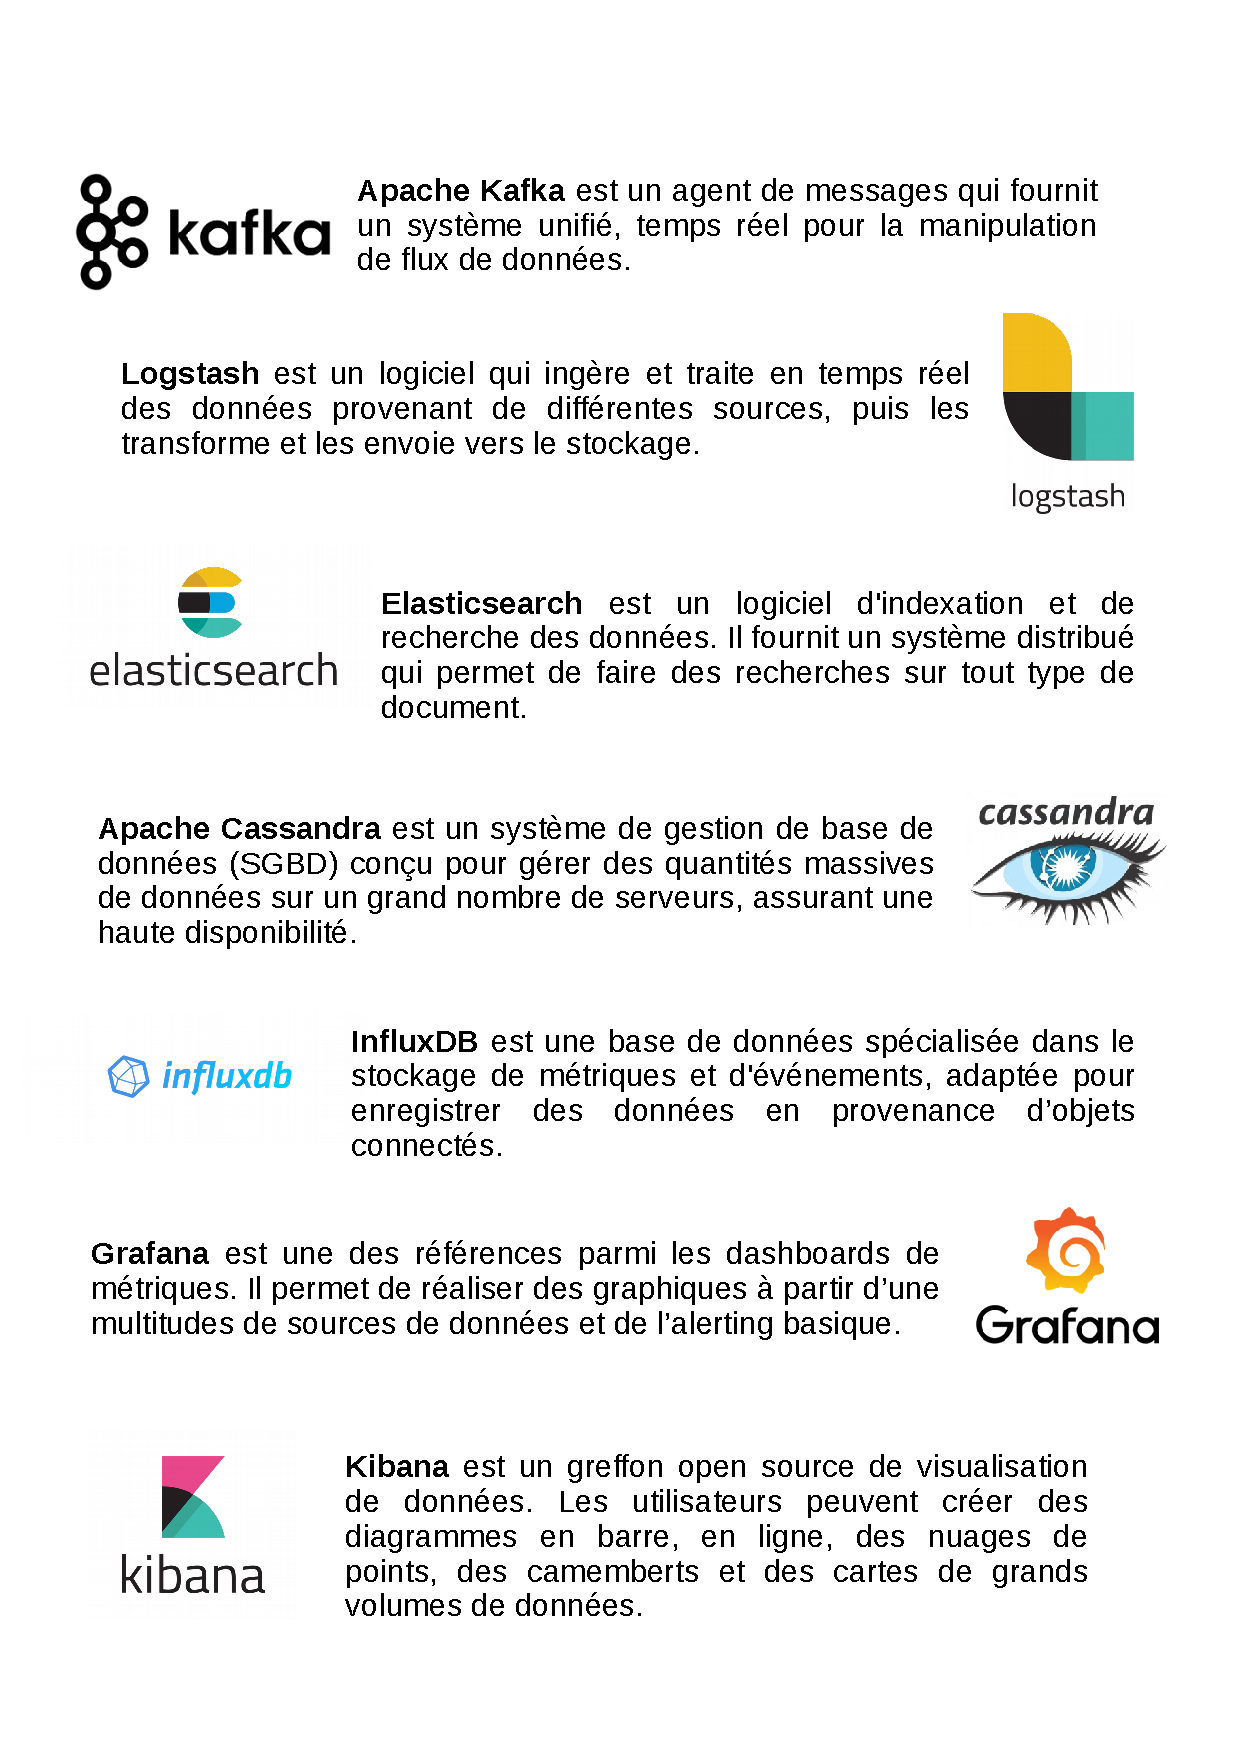
\includegraphics[width=16cm]{pdfinc/Outils.pdf}
\subsection{Google Developer: ARCore}
Nous nous sommes également penché sur une technologie assez recente qui a un profond interêt dans le cadre de notre projet puisqu'il
s'agit de l'intégration de Motion Tracking et la profondeur de champ. Un outil parfaitement adapté par exemple pour les scans de superficie
ou de visite virtuel.
\href{https://www.youtube.com/watch?v=NhJydpMkpug}{ARCore Google Developer Video}


\chapter{Conclusion}
\section{Faisabilité technique}
Avec la multitude d'outils open-source que nous utilisons, certains coût s'amoindrisse. Néanmoins une Infrastructure
Big Data nécessite des ressources assez conséquente pour fonctionner dans de bonnes conditions et assurer une haute
disponibilité. De ce fait il est important d'avoir des techniciens qualifiés pour accomplir ce genre de projet.
Temps estimé de la solution : 14-16 mois (avec un cahier des charges bien définis et une roadmap bien fixée)


\section{Impact social}
On peut se poser la question de l'impact social.
En effet en 2010 les 55 400 entreprises du secteur immobilier représentaient
112 000 emplois, pour un CA HT de 15,4 Md \euro{}
\footnote{Source: \url{https://fr.wikipedia.org/wiki/Agent_immobilier}}.

La transformation engrangé par un tel projet risque de détruire beaucoup
d'emplois et en dé-localisé d'autre, ainsi que de voir l'économie principalement
local du secteur se centralisé dans les grandes villes. Sans pour autant voir de
net amélioration du secteur économique. 

\end{document}
